In this section we conduct a thorough investigation of WSDDN and its components on weakly supervised detection and image classification.

\subsection{Benchmark data.}
We evaluate our method on the PASCAL VOC 2007 and 2010 datasets \cite{Everingham10}, as they are the most widely-used benchmark in weakly supervised object detection. While the VOC 2007 dataset consists of 2501 training, 2510 validation, and 5011 test images containing bounding box annotations for 20 object categories, VOC 2010 dataset contains 4998 training, 5105 validation, and 9637 test images for the same number of categories. We use the suggested training and validation splits and report results evaluated on \emph{test} split. We report performance of our method on both the object detection and the image classification tasks of PASCAL VOC. 

For detection, we use two performance measures. The first one follows the standard PASCAL VOC protocol and reports average precision (AP) at  $50\%$ intersection-over-union (IoU) of the detected boxes with the ground truth ones. We also report CorLoc, a commonly-used weakly supervised detection measure~\cite{Deselaers12}. CorLoc is the percentage of images that contain at least one instance of the target object class for which the most confident detected bounding box overlaps by at least $50\%$ with one of these instances. Differently from AP, which is measured on the PASCAL test set, CorLoc is evaluated on the union of the training and validation subset of PASCAL. For classification, we use the standard PASCAL VOC protocol and report AP.

\subsection{Experimental setup.}\label{subsec:expsetup}
We comprehensively evaluate our method with three pre-trained CNN models in our experiments as in~\cite{Girshick15}. The first network is the VGG-CNN-F~\cite{Chatfield14} which is similar to AlexNet~\cite{Krizhevsky12} but has reduced number of convolutional filters. We refer to this network as \textbf{S}, for small. The second one is VGG-CNN-M-1024 which has the same depth as \textbf{S} but has smaller stride in the first convolutional layer. We name this network \textbf{M} for medium. The last network is the deep VGG-VD16 model~\cite{Simonyan15} and we call this network \textbf{L} for large. These models, which are pre-trained on the ImageNet ILSVRC 2012 challenge data \cite{Russakovsky15}, attain  $18.8 \%$, $16.1 \%$ and $9.9 \%$ top-5 accuracy respectively (using a single centre-crop) on ILSVRC (importantly no bounding box information is provided during pre-training). As explained in \cref{s:pretrained}, we apply the following modifications to the network. First, we replace the last pooling layer \textit{pool5} with a SPP layer~\cite{He14} which is configured to be compatible with the network's first fully connected layer. Second, we add a parallel detection branch to the classification one that contains a fully-connected layer followed by a soft-max layer. Third, we combine the classification and detection streams by element-wise product followed by summing scores across regions, and feed the latter to a binary log-loss layer. Note that this layer assesses the classification performance for the 20 classes together, but each of them is treated as a different binary classification problem; the reason is that classes can co-occur in the PASCAL VOC, such that the softmax log loss used in AlexNet is not appropriate.

The WSDDNs are trained on the PASCAL VOC training and validation data by using fine-tuning on all layers, a widely-adopted technique to improve the performance of a CNN on a target domain~\cite{Chatfield14}. Here, however, fine tuning performs the essential function of learning the classification and detection streams, effectively causing the network to learn to detect objects, but using only weak image-level supervision. The experiments are run for $20$ epochs and all the layers are fine-tuned with the learning rate $10^{-5}$ for the first ten epochs and $10^{-6}$ for the last ten epochs. Each minibatch contains all region proposals from a single image.

In order to generate candidate regions to use with our networks, we evaluate two proposal methods, Selective Search Windows (SSW)~\cite{Sande11} using its \textit{fast} setting, and EdgeBoxes (EB)~\cite{Zitnick14}. In addition to region proposals, EB provides an objectness score for each region based on the number of contours wholly encloses. We exploit this additional information by multiplying the feature map $\phi_{\text{SPP}}$ proportional to its score via a scaling layer in WSDDN and denote this setting as \emph{Box Sc}. Since we use a SPP layer to aggregate descriptors for each region, images do not need to be resized to a particular size as in the original pre-trained model. Instead, we keep the original aspect ratio of images fixed and resize them to five different scales (setting their maximum of width or height to $\lbrace 480,576,688,864,1200\rbrace$ respectively) as in \cite{He14}. During training, we apply random horizontal flips to the images and select a scale at random as a form of jittering or data augmentation. At test time we average the outputs of 10 images (\ie the 5 scales and their flips). We use the publicly available CNN toolbox MatConvNet~\cite{Vedaldi15} to conduct our experiments and share our code, models and data~\footnote{\url{https://github.com/hbilen/WSDDN}}.

When evaluated on an image, WSDDN produces, for each target class $c$ and image $\bx$, a score $\bx^\mathcal{R}_r = S_c(\bx;r)$ for each region $r$ and an aggregated score $y_c=S_c(\bx)$ for each image. Non-maxima suppression (with $40$ \% IoU threshold) is applied to the regions and then the scored regions and images are pooled together to compute detection AP and CorLoc.

 \begin{table}
% table 2
\begin{center}
\begin{tabular}{lccc|c}
& \textbf{S} & \textbf{M} & \textbf{L} & \textbf{Ens.}\\
\toprule
SSW                                       & 31.1 & 30.9 & 24.3 & 33.3 \\
EB                                        & 31.5 & 30.9 & 25.5 & 34.2 \\
EB + Box Sc. & 33.4 & 32.7 & 30.4 & 36.7\\
EB + Box Sc. + Sp. Reg.        & \bf{34.5} & \bf{34.9} & \bf{34.8} & \bf{39.3} \\
\end{tabular}
\vspace{0.2em}
\caption{{\bf VOC 2007 test} detection average precision (\%). The ensemble network is denoted as \textbf{Ens}.}
 \label{tab:voc2007base}
\end{center}
\end{table}



\begin{table*}[t!]
\centering
\renewcommand{\arraystretch}{1.2}
\renewcommand{\tabcolsep}{1.2mm}
\resizebox{\linewidth}{!}{
  \begin{tabular}{@{}L{3.5cm}|*{20}{x}|x@{}}
method & aero      & bike      & bird      & boat      & bottle     & bus        & car        & cat        & chair      & cow        & table      & dog        & horse      & mbike      & persn     & plant      & sheep      & sofa       & train      & tv         & mean       \\
\toprule
WSDDN \textbf{S} & 42.9 & 56.0 & 32.0 & 17.6 & 10.2 & 61.8 & 50.2 & 29.0 & 3.8 & 36.2 & 18.5 & 31.1 & \bf{45.8} & 54.5 & 10.2 & 15.4 & 36.3 & 45.2 & 50.1 & 43.8 & 34.5\\
WSDDN \textbf{M} & 43.6 & 50.4 & 32.2 & \bf{26.0} &  9.8 & 58.5 & 50.4 & 30.9 & 7.9 & 36.1 & 18.2 & 31.7 & 41.4 & 52.6 & 8.8 & 14.0 & 37.8 & 46.9 & 53.4 & 47.9 & 34.9\\ 
WSDDN \textbf{L} & 39.4 & 50.1 & 31.5 & 16.3 & 12.6 & 64.5 & 42.8 & \bf{42.6} & 10.1 & 35.7 & 24.9 & 38.2 & 34.4 & 55.6 & 9.4 & 14.7 & 30.2 & 40.7 & 54.7 & 46.9 & 34.8\\ 
WSDDN Ensemble   & 46.4 & \bf{58.3} & \bf{35.5} & {25.9} & \bf{14.0} & \bf{66.7} & \bf{53.0} & {39.2} & 8.9 & \bf{41.8} & \bf{26.6} & \bf{38.6} & {44.7} & \bf{59.0} & 10.8 & 17.3 & \bf{40.7} & \bf{49.6} & \bf{56.9} & \bf{50.8} & \bf{39.3} \\
\midrule
Bilen \etal \cite{Bilen14} & 42.2 & 43.9 & 23.1 &  9.2 & {12.5} & {44.9} & 45.1 & 24.9 &  8.3 & 24.0 & 13.9 & 18.6 & 31.6 & 43.6 &  7.6 & \bf{20.9} & 26.6 & 20.6 & 35.9 & 29.6 & 26.4\\ 
Bilen \etal \cite{Bilen15} & 46.2 & 46.9 & {24.1} & {16.4} & {12.2} & 42.2 & {47.1} & 35.2 &  7.8 & 28.3 & 12.7 & 21.5 & 30.1 & 42.4 &  7.8 & {20.0} & {26.8} & 20.8 & {35.8} & 29.6 & 27.7\\
Cinbis \etal \cite{Cinbis15} & 39.3 & 43.0 & 28.8 & 20.4 &  8.0 & 45.5 & 47.9 & 22.1 & 8.4 & 33.5 & 23.6 & 29.2 & 38.5 & 47.9 & \bf{20.3} & 20.0 & 35.8 & 30.8 & 41.0 & 20.1 & 30.2 \\
Wang \etal \cite{Wang14a} & {48.8} & 41.0 & 23.6 & 12.1 & 11.1 & 42.7 & 40.9 & {35.5} & \bf{11.1} & {36.6} & {18.4} & {35.3} & {34.8} & {51.3} & {17.2} & 17.4 & {26.8} & {32.8} & 35.1 & {45.6} & {30.9}\\
Wang \etal \cite{Wang14a}+context & \bf{48.9} & 42.3 & 26.1 & 11.3 & 11.9 & 41.3 & 40.9 & 34.7 & 10.8 & 34.7 & 18.8 & 34.4 & 35.4 & 52.7 & 19.1 & 17.4 & 35.9 & 33.3 & 34.8 & 46.5 & 31.6\\
\end{tabular}
}
\vspace{0.2em}
\caption{{\bf VOC 2007 test} detection average precision (\%). Comparison of our WSDDN on PASCAL VOC 2007 to the state-of-the-art in terms of AP.}
 \label{tab:voc2007ap}
\end{table*}



\begin{table*}[t!]
\centering
\renewcommand{\arraystretch}{1.2}
\renewcommand{\tabcolsep}{1.2mm}
\resizebox{\linewidth}{!}{
  \begin{tabular}{@{}L{3.5cm}|*{20}{x}|x@{}}
    method & aero      & bike      & bird      & boat      & bottle     & bus        & car        & cat        & chair      & cow        & table      & dog        & horse      & mbike      & persn     & plant      & sheep      & sofa       & train      & tv         & mean       \\
    \midrule
    WSDDN \bf{S} & 68.5 & 67.5 & 56.7 & 34.3 & 32.8 & 69.9 & 75.0 & 45.7 & 17.1 & 68.1 & 30.5 & 40.6 & 67.2 & 82.9 & 28.8 & 43.7 & 71.9 & 62.0 & 62.8 & 58.2 & 54.2\\
    WSDDN \bf{M} & 65.1 & 63.4 & 59.7 & {45.9} & 38.5 & 69.4 & 77.0 & 50.7 & 30.1 & \bf{68.8} & 34.0 & 37.3 & 61.0 & 82.9 & 25.1 & 42.9 & \bf{79.2} & 59.4 & \bf{68.2} & 64.1 & 56.1\\
    WSDDN \bf{L} & 65.1 & 58.8 & 58.5 & 33.1 & 39.8 & 68.3 & 60.2 & \bf{59.6} & \bf{34.8} & 64.5 & 30.5 & 43.0 & 56.8 & 82.4 & 25.5 & 41.6 & 61.5 & 55.9 & 65.9 & 63.7 & 53.5\\
    WSDDN Ensemble & 68.9 & \bf{68.7} & \bf{65.2} & 42.5 & \bf{40.6} & \bf{72.6} & {75.2} & {53.7} & {29.7} & {68.1} & {33.5} & {45.6} & {65.9} & \bf{86.1} & {27.5} & \bf{44.9} & {76.0} & \bf{62.4} & {66.3} & \bf{66.8} &\bf{58.0}\\
    \midrule
    Bilen \etal \cite{Bilen15}    & 66.4 & 59.3 & 42.7 & 20.4 & {21.3} & {63.4} & {74.3} & \bf{59.6} & 21.1 & {58.2} & 14.0 & 38.5 & 49.5 & 60.0 & 19.8 & {39.2} & 41.7 & 30.1 & 50.2 & 44.1 & 43.7\\
    Cinbis \etal \cite{Cinbis15} & 65.3 & 55.0 & 52.4 & \bf{48.3} & 18.2 & 66.4 & \bf{77.8} & 35.6 & 26.5 & 67.0 & \bf{46.9} & \bf{48.4} & \bf{70.5} & 69.1 & \bf{35.2} & 35.2 & 69.6 & 43.4 & 64.6 & 43.7 & 52.0 \\
    Wang \etal \cite{Wang14a}     & \bf{80.1} & {63.9} & {51.5} & 14.9 & 21.0 & 55.7 & 74.2 & 43.5 & {26.2} & 53.4 & 16.3 & 56.7 & {58.3} & {69.5} & 14.1 & 38.3 & {58.8} & {47.2} & 49.1 & {60.9} & {48.5}\\
  \end{tabular}
  }
  \vspace{0.2em}
  \caption{{\bf VOC 2007 trainval} correct localization (CorLoc \cite{Deselaers12}) on positive \textit{trainval} images (\%).}
  \label{tab:voc2007corloc}
\end{table*}

% classification results %
\begin{table*}[t!]
\centering
\renewcommand{\arraystretch}{1.2}
\renewcommand{\tabcolsep}{1.2mm}
\resizebox{\linewidth}{!}{
  \begin{tabular}{@{}L{3.5cm}|*{20}{x}|x@{}}
method & aero      & bike      & bird      & boat      & bottle     & bus        & car        & cat        & chair      & cow        & table      & dog        & horse      & mbike      & persn     & plant      & sheep      & sofa       & train      & tv         & mean       \\
\midrule
WSDDN \bf{S}   & 92.5 & 89.9 & 89.5 & 88.3 & 66.5 & 83.6 & 92.1 & 90.3 & 73.0 & 85.7 & 72.6 & 91.4 & 90.1 & 89.0 & 94.4 & 78.1 & 86.0 & 76.1 & 91.1 & 85.5 & 85.3\\
WSDDN \bf{M}   & 93.9 & 91.0 & 90.4 & 89.3 & 72.7 & 86.4 & 91.9 & 91.5 & 73.8 & 85.6 & 74.9 & 91.9 & 91.5 & 89.9 & 94.5 & 78.6 & 85.0 & 78.6 & 91.5 & 85.7 & 86.4\\ 
WSDDN \bf{L}   & 93.3 & \bf{93.9} & 91.6 & \bf{90.8} & \bf{82.5} & \bf{91.4} & \bf{92.9} & \bf{93.0} & 78.1 & \bf{90.5} & \bf{82.3} & \bf{95.4} & \bf{92.7} & 92.4 & 95.1 & \bf{83.4} & \bf{90.5} & 80.1 & 94.5 & \bf{89.6} & \bf{89.7}\\
WSDDN Ensemble & 95.0 & 92.6 & 91.2 & 90.4 & 79.0 & 89.2 & 92.8 & 92.4 & \bf{78.5} & \bf{90.5} & 80.4 & 95.1 & 91.6 & \bf{92.5} & 94.7 & 82.2 & 89.9 & \bf{80.3} & 93.1 & 89.1 & 89.0\\
\midrule
Oquab \etal \cite{Oquab14} &  88.5  &  81.5  &  87.9  &  82.0  &  47.5  &  75.5  &  90.1  &  87.2  &  61.6  &  75.7  &  67.3 &  85.5 &  83.5 &  80.0 &  \bf{95.6} &  60.8 &  76.8 &  58.0 &  90.4  &  77.9  &  77.7 \\
SPP \cite{He14} & -- &  -- & -- & -- & -- & -- & -- & -- & -- & -- & -- & -- & -- & -- & -- & -- & -- & -- & -- & -- & 82.4 \\
VGG-F \cite{Chatfield14} &  88.7 & 83.9 & 87.0 & 84.7 & 46.9 & 77.5 &  86.3 & 85.4 & 58.6 & 71.0 & 72.6 & 82.0 & 87.9 & 80.7 & 91.8 & 58.5 & 77.4 & 66.3 &  89.1 & 71.3 & 77.4\\
VGG-M-1024 \cite{Chatfield14} & 91.4 & 86.9 & 89.3 & 85.8 & 53.3 & 79.8 & 87.8 & 88.6 & 59.0 & 77.2 & 73.1 & 85.9 & 88.3 & 83.5 & 91.8 & 59.9 & 81.4 & 68.3 & 93.0 & 74.1 & 79.9\\
VGG-S \cite{Chatfield14} &  \bf{95.3} & {90.4} & \bf{92.5} & {89.6} & 54.4 & 81.9 & {91.5} & {91.9} & 64.1 & 76.3 & 74.9 & {89.7} & {92.2} & {86.9} & {95.2} & 60.7 & 82.9 & 68.0 & \bf{95.5} & 74.4 & 82.4\\
VGG-VD16 \cite{Simonyan15} & -- &  -- & -- & -- & -- & -- & -- & -- & -- & -- & -- & -- & -- & -- & -- & -- & -- & -- & -- & -- & 89.3 \\ 
\bottomrule
\end{tabular}
}
\vspace{0.05em}
\caption{{\bf VOC 2007 test} classification average precision (\%).}
 \label{tab:voc2007cls}
\end{table*}

\begin{table*}[t!]
\centering
\renewcommand{\arraystretch}{1.2}
\renewcommand{\tabcolsep}{1.2mm}
\resizebox{\linewidth}{!}{
  \begin{tabular}{@{}L{3.5cm}|*{20}{x}|x@{}}
    method & aero      & bike      & bird      & boat      & bottle     & bus        & car        & cat        & chair      & cow        & table      & dog        & horse      & mbike      & persn     & plant      & sheep      & sofa       & train      & tv         & mean       \\
    \midrule
    WSDDN Ensemble                      & \bf{57.4} & \bf{51.8} & \bf{41.2} & \bf{16.4} & \bf{22.8} & \bf{57.3} & \bf{41.8} & \bf{34.8} & \bf{13.1} & \bf{37.6} & 10.8 & \bf{37.0} & \bf{45.2} & \bf{64.9} & 14.1 & \bf{22.3} & \bf{33.8} & \bf{27.6} & \bf{49.1} & \bf{44.8} & \bf{36.2}\\
    \midrule
    Cinbis \etal \cite{Cinbis15} & 44.6 & 42.3 & 25.5 & 14.1 & 11.0 & 44.1 & 36.3 & 23.2 & 12.2 & 26.1 & \bf{14.0} & 29.2 & 36.0 & 54.3 & \bf{20.7} & 12.4 & 26.5 & 20.3 & 31.2 & 23.7 & 27.4\\
  \end{tabular}
  }
  \vspace{0.2em}
  \caption{{\bf VOC 2010 test} detection average precision (\%). \url{http://host.robots.ox.ac.uk:8080/anonymous/3QGEGM.html}}
  \label{tab:voc2010ap}
\end{table*}

\begin{table*}[t!]
\centering
\renewcommand{\arraystretch}{1.2}
\renewcommand{\tabcolsep}{1.2mm}
\resizebox{\linewidth}{!}{
  \begin{tabular}{@{}L{3.5cm}|*{20}{x}|x@{}}
    method & aero      & bike      & bird      & boat      & bottle     & bus        & car        & cat        & chair      & cow        & table      & dog        & horse      & mbike      & persn     & plant      & sheep      & sofa       & train      & tv         & mean       \\
    \midrule
    WSDDN Ensemble & \bf{77.4} & \bf{73.2} & \bf{61.9} & 39.6 & \bf{50.8} & \bf{84.4} & 67.5 & \bf{49.6} & 38.6 & \bf{73.4} & 30.4 & \bf{53.2} & 72.9 & \bf{84.1} & 30.3 & \bf{53.1} & \bf{76.6} & 48.5 & 61.6 & \bf{66.7} & \bf{59.7}\\
    \midrule
    Cinbis \etal \cite{Cinbis15} &  61.1 & 65.0 & 59.2 & \bf{44.3} & 28.3 & 80.6 & \bf{69.7} & 31.2 & \bf{42.8} & 73.3 & \bf{38.3} & 50.2 & \bf{74.9} & 70.9 & \bf{37.3} & 37.1 & 65.3 & \bf{55.3} & \bf{61.7} & 58.2 & 55.2\\
  \end{tabular}
  }
  \vspace{0.2em}
  \caption{{\bf VOC 2010 trainval} correct localization (CorLoc \cite{Deselaers12}) on positive \textit{trainval} images (\%).}
  \vspace{2em}
  \label{tab:voc2010corloc}
\end{table*}


% --------------------------------------------------------------------------------------
\subsection{Detection results}\label{s:detres}
% --------------------------------------------------------------------------------------

\paragraph{Baseline method.} First we design a single stream classification-detection network as an alternative baseline to WSDDN. Part of the construction is similar to WSDDN, as we replace \textit{pool5} layer of VGG-CNN-F model with an SPP. However, we do not branch off two streams, but simply append to the last fully connected layer ($\phi_\text{fc8c}$) the following loss layer \[
\frac{1}{nC}
\sum_{i=1}^n
\sum_{k=1}^C
\max\{0, 1 - y_{ki} \log \sum_{r=1}^{|\mathcal{R}|} \exp(x^{\mathcal{R}}_{cr})\}.
\]
The term $\log \sum_{r=1}^{|\mathcal{R}|} \exp(x^{\mathcal{R}}_{cr}$) is a soft approximation of the max operator $\max_r x_{cr}^\mathcal{R}$ and was found to yield better performance than using the max scoring region. This observation is also reported in \cite{Bilen14}. Note that the non-linearity is necessary as otherwise aggregating region-based scores would sum over the scores of a majority of regions that are uninformative. The loss function is once more a sum of $C$ binary hinge-losses, one for each class. This baseline obtains $21.6 \%$ mAP detection score on the PASCAL VOC test set, which is well below the state-of-the-art ($31.6 \%$ in~\cite{Wang14a}).

\paragraph{Pre-trained CNN architectures.} We evaluate our method with the models \textbf{S}, \textbf{M} and \textbf{L} and also report the results for the ensemble of these models by simply averaging their scores. Table~\ref{tab:voc2007base} shows that WSDDN with individual models \textbf{S} and \textbf{M} are already on par with the state-of-the-art method~\cite{Wang14a} and the ensemble outperforms the best previous score in the VOC 2007 dataset. Differently from supervised detection methods (\eg \cite{Girshick15}), detection performance of WSDDN does not improve with use of wider or deeper networks. In contrast, model \textbf{L} performs significantly worse than models \textbf{S} and \textbf{M} (see~\cref{tab:voc2007base}). This can be explained with the fact that model~\textbf{L} frequently focuses on parts of objects, instead of whole instances, and is still able to associate these parts with object categories due to its smaller convolution strides, higher resolution and deeper architecture.

\paragraph{Object proposals.} Next, we compare the detection performances with two popular object proposal methods, SSW~\cite{Sande11} and EB~\cite{Zitnick14}. While both the region proposals provides comparable quality region proposals, using box scores of EB (denoted as \emph{Box Sc} in~\cref{tab:voc2007base}) leads to a $~2\%$ improvement for models \textbf{S} and \textbf{M} and boosts the detection performance of model \textbf{L} $~5\%$.

\paragraph{Spatial regulariser.} We denote the setting where WSDDN is trained with the additional spatial regularisation term (denoted as \emph{Sp. Reg.} in \cref{tab:voc2007base}). Finally the introduction of the regularisation improves the detection performance $1$, $2$ and $4$ mAP points for models \textbf{S}, \textbf{M} and \textbf{L} respectively. The improvements show that larger network benefits more from introduction of the spatial invariance around high confidence regions.


\paragraph{Comparison with the state of the art.}
After evaluating the design decisions, we follow the best setting (last row in \cref{tab:voc2007base}) and compare WSDDN to the state of the art in weakly supervised detection literature in \cref{tab:voc2007ap} and \cref{tab:voc2007corloc} for the VOC 2007 dataset and in \cref{tab:voc2010ap} and \cref{tab:voc2010corloc} for the VOC 2010 dataset. The results show that our method already achieves overall significantly better performance than these alternatives with a single model and ensemble models further boost the performance. The majority of previous work \cite{Song14,Song14a,Bilen14,Wang14,Bilen15} use the Caffe reference CNN model \cite{Jia13}, which is comparable to model~\textbf{S} in this paper, as a black box to extract features over SSW proposals. In addition to CNN features, Cinbis \etal \cite{Cinbis15} use Fisher Vectors~\cite{Perronnin10a} and EB objectness measure of Zitnick and Dollar \cite{Zitnick14} as well. Differently from the previous work, WSDDN is based on a simple modification of the original CNN architecture fine-tuned on the target data using back-propagation.

Next, we investigate the results in more detail. While our method significantly outperforms the alternatives in majority of categories, is not as strong in chair, person and pottedplant categories. Failure and success case are illustrated in \cref{fig:detexamples}. It can be noted that, by far, the most important failure modality for our system is that an object part (e.g. person face) is detected instead as the object as a whole. This can be explained by the fact that parts such as ``face'' are very often much more discriminative and with a less variable appearance than the rest of the object. Note that the root cause for this failure modality is that we, as many other authors, define objects as image regions that are most predictive for a given object class, and these may not include the object as a whole. Addressing this issue will therefore require incorporating additional cue in the model to try to learn the ``whole object''.

The output of our model could also be used as input to one of the existing methods for weakly-supervised detection that use a CNN as a black-box for feature extraction. Investigating this option is left to future work.

\begin{figure*}[t!]
%\begin{center}
\begin{tabular}{*{6}{C{0.13\textwidth}}}
  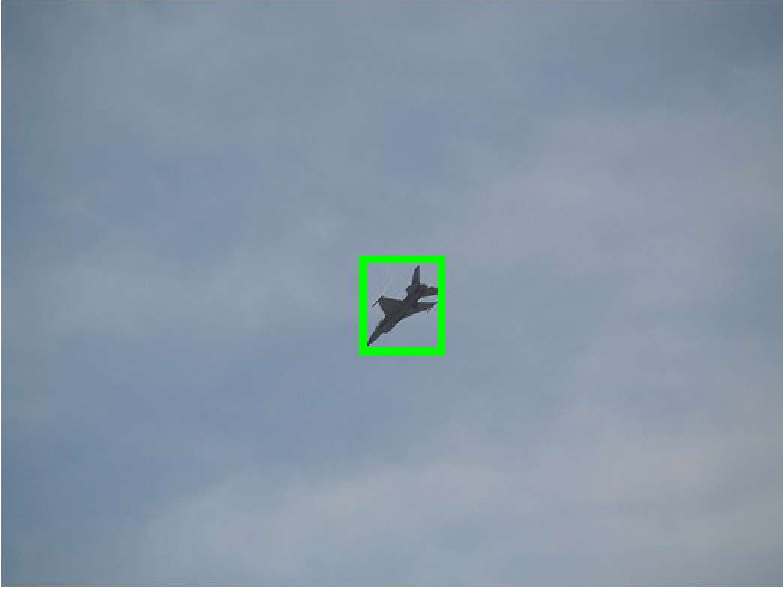
\includegraphics[height=0.12\textwidth,width=0.15\textwidth]{aeroplane_pos_000216.pdf}&
  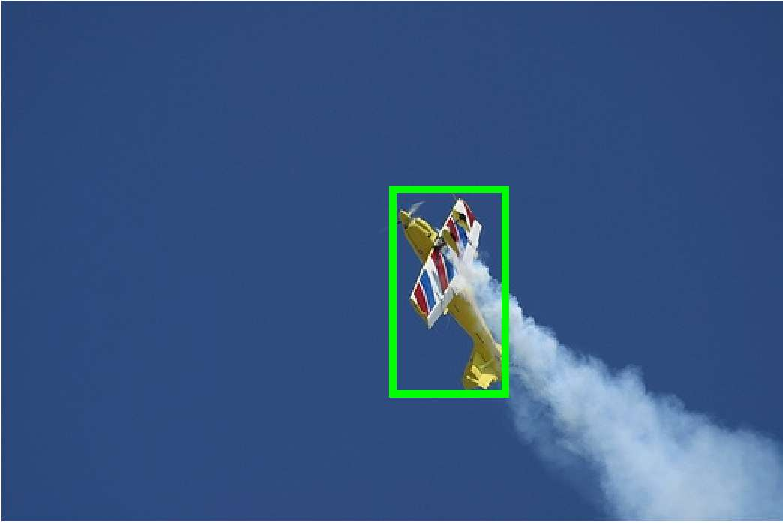
\includegraphics[height=0.12\textwidth,width=0.15\textwidth]{aeroplane_pos_000521.pdf}&
  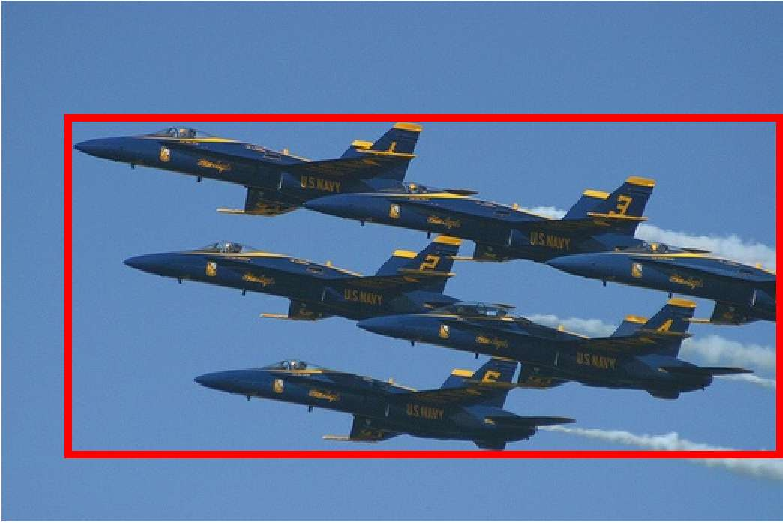
\includegraphics[height=0.12\textwidth,width=0.15\textwidth]{aeroplane_neg_002217.pdf}&
  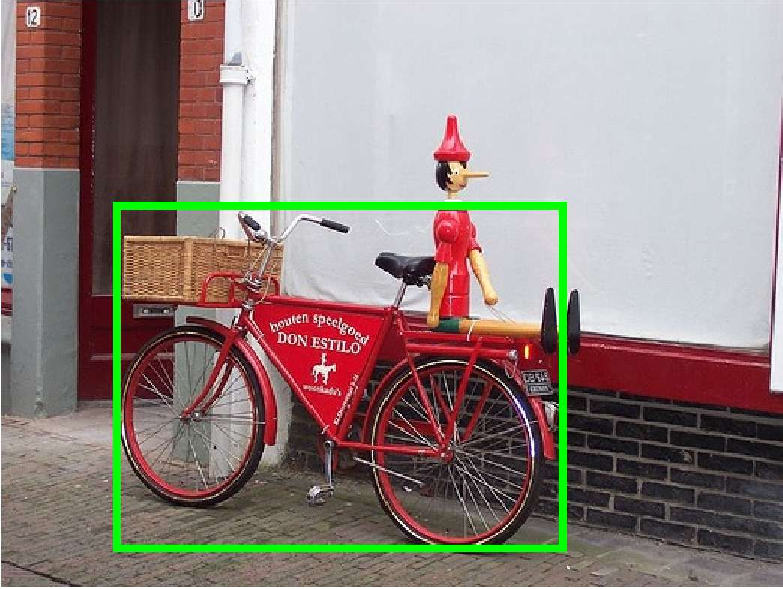
\includegraphics[height=0.12\textwidth,width=0.15\textwidth]{bicycle_pos_000015.pdf}&
  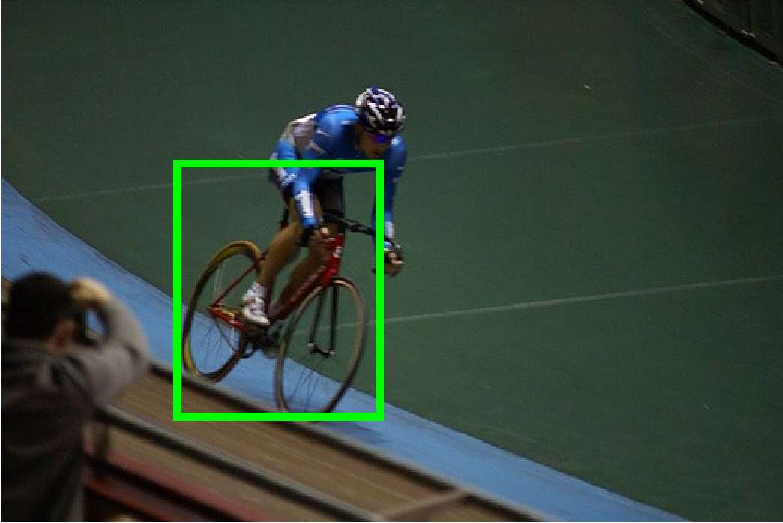
\includegraphics[height=0.12\textwidth,width=0.15\textwidth]{bicycle_pos_000139.pdf}&
  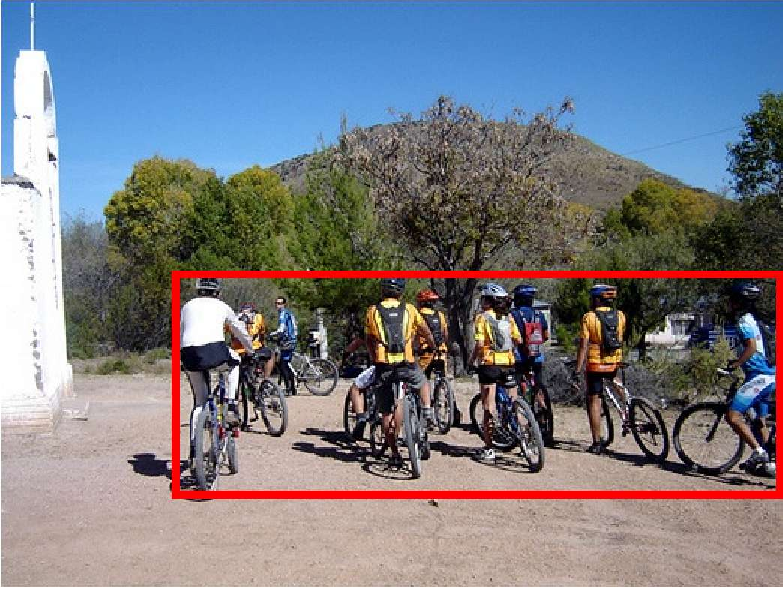
\includegraphics[height=0.12\textwidth,width=0.15\textwidth]{bicycle_neg_002168.pdf}\\[-2ex]

  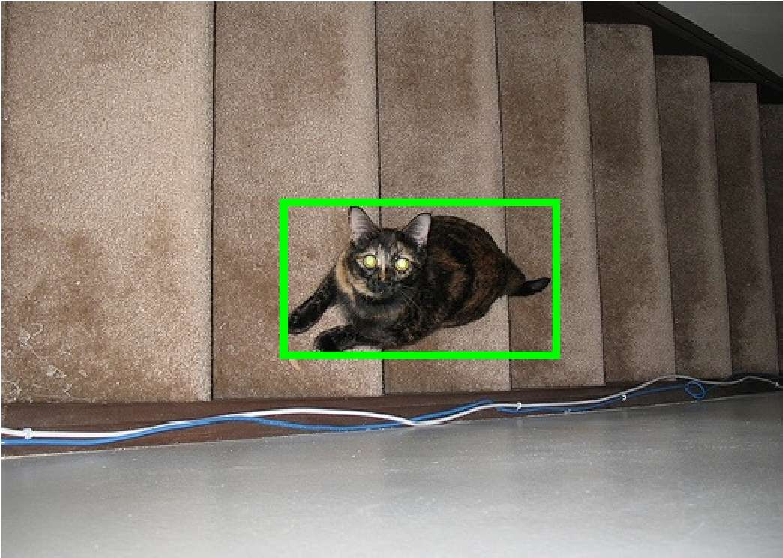
\includegraphics[height=0.12\textwidth,width=0.15\textwidth]{cat_pos_000049.pdf}&
  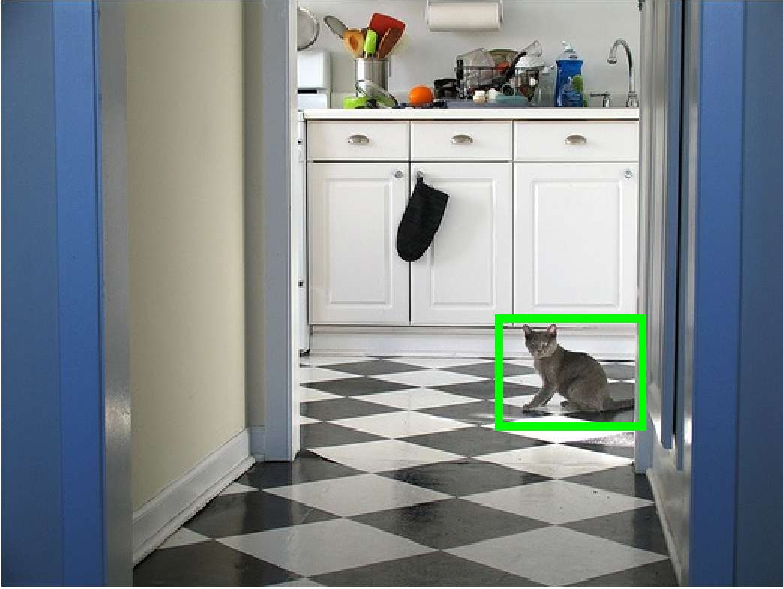
\includegraphics[height=0.12\textwidth,width=0.15\textwidth]{cat_pos_000146.pdf}&
  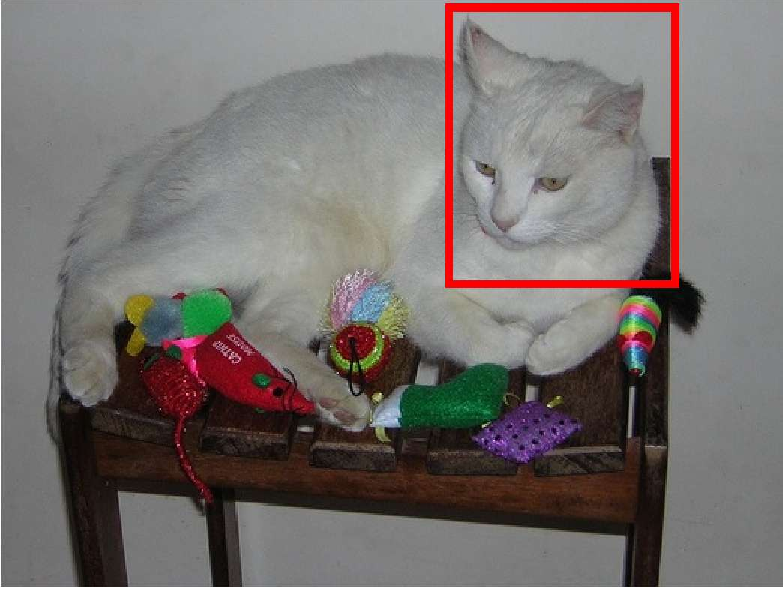
\includegraphics[height=0.12\textwidth,width=0.15\textwidth]{cat_neg_000053.pdf}&
  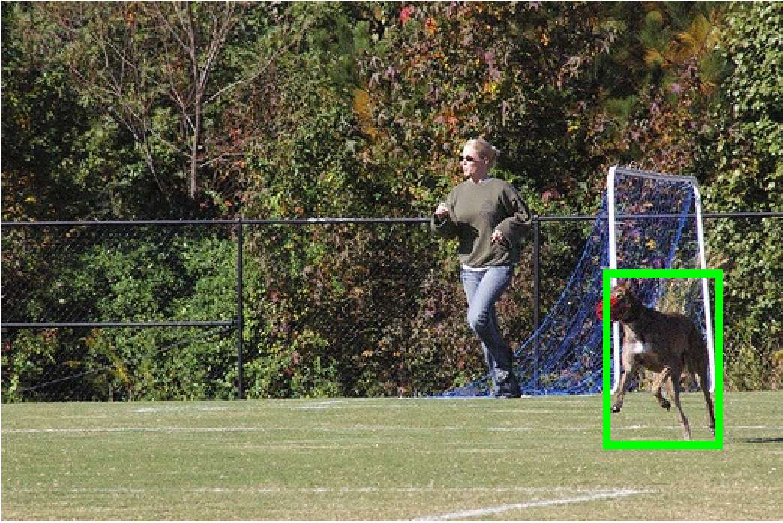
\includegraphics[height=0.12\textwidth,width=0.15\textwidth]{dog_pos_000734.pdf}&
  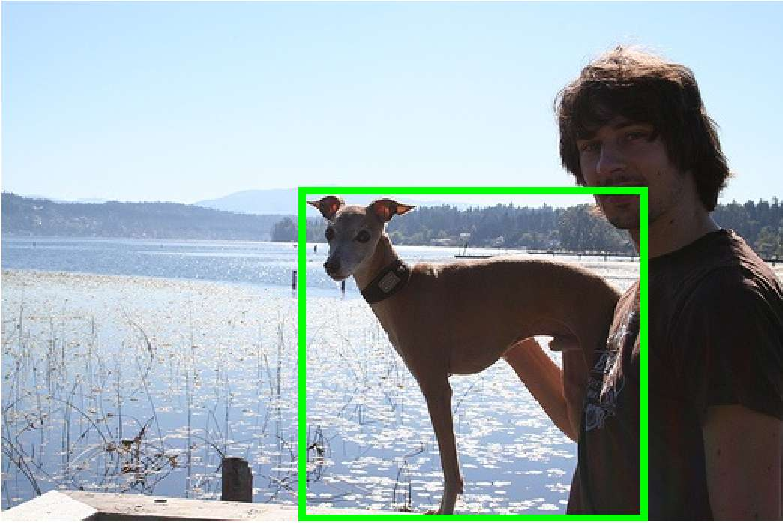
\includegraphics[height=0.12\textwidth,width=0.15\textwidth]{dog_pos_000258.pdf}&
  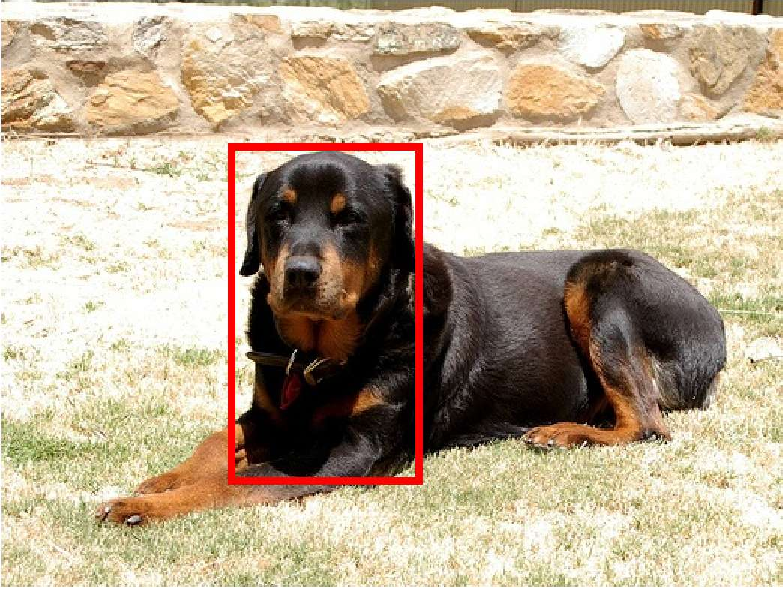
\includegraphics[height=0.12\textwidth,width=0.15\textwidth]{dog_neg_000037.pdf}\\[-2ex]
  
  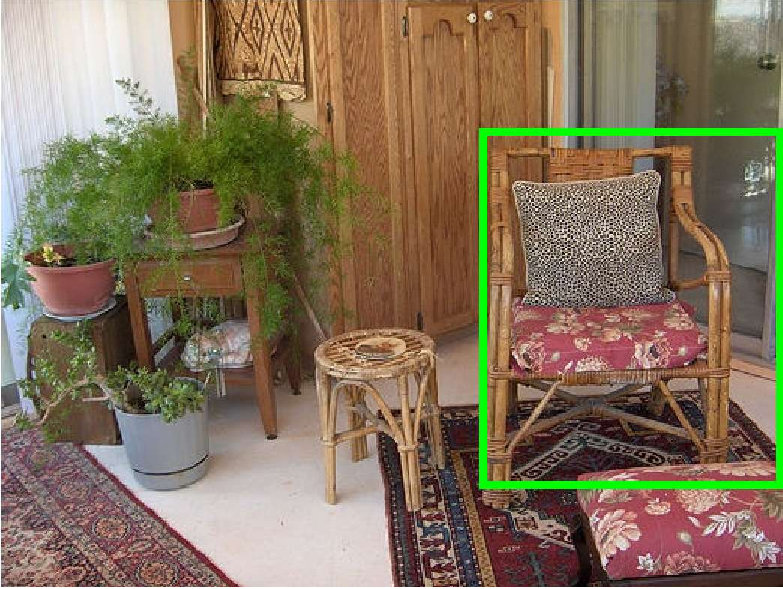
\includegraphics[height=0.12\textwidth,width=0.15\textwidth]{chair_pos_000234.pdf}&
  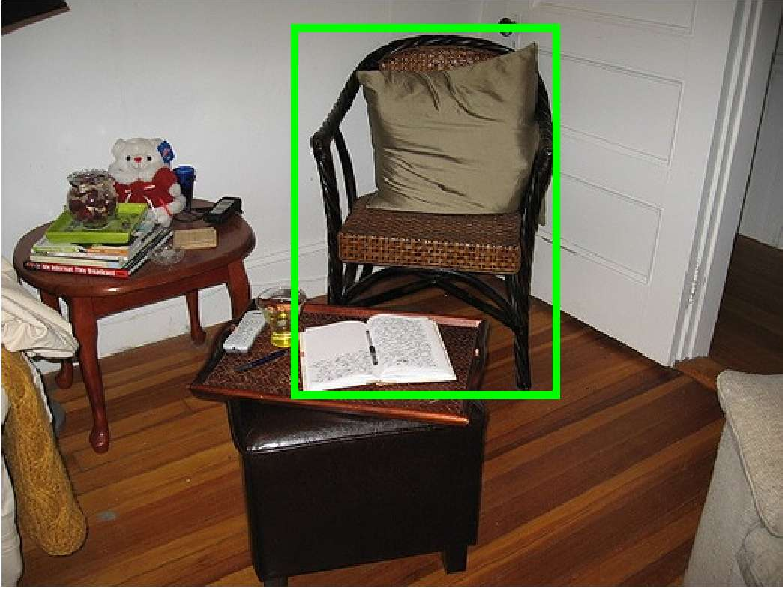
\includegraphics[height=0.12\textwidth,width=0.15\textwidth]{chair_pos_000008.pdf}&
  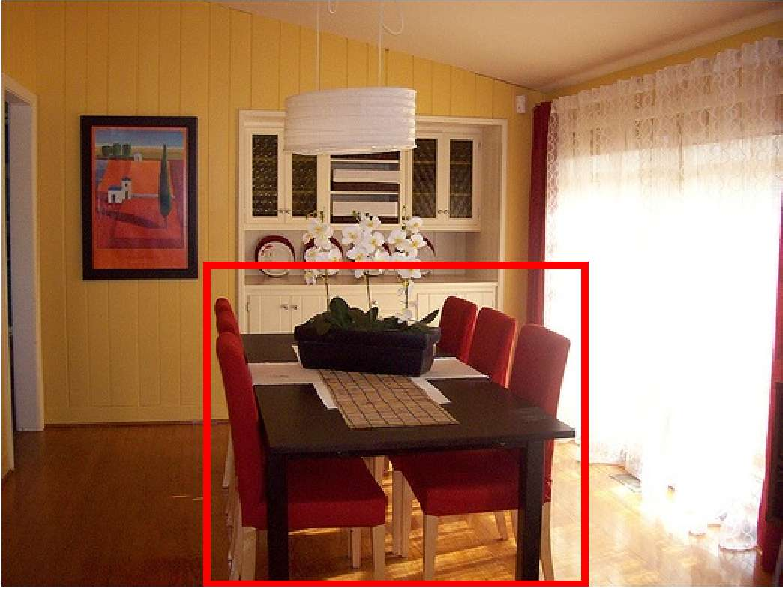
\includegraphics[height=0.12\textwidth,width=0.15\textwidth]{chair_neg_000006.pdf}&
  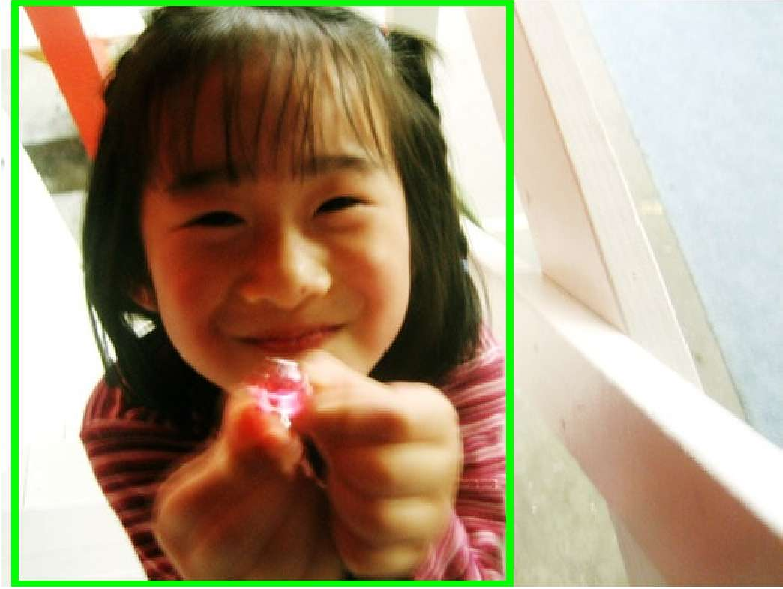
\includegraphics[height=0.12\textwidth,width=0.15\textwidth]{person_pos_000664.pdf}&
  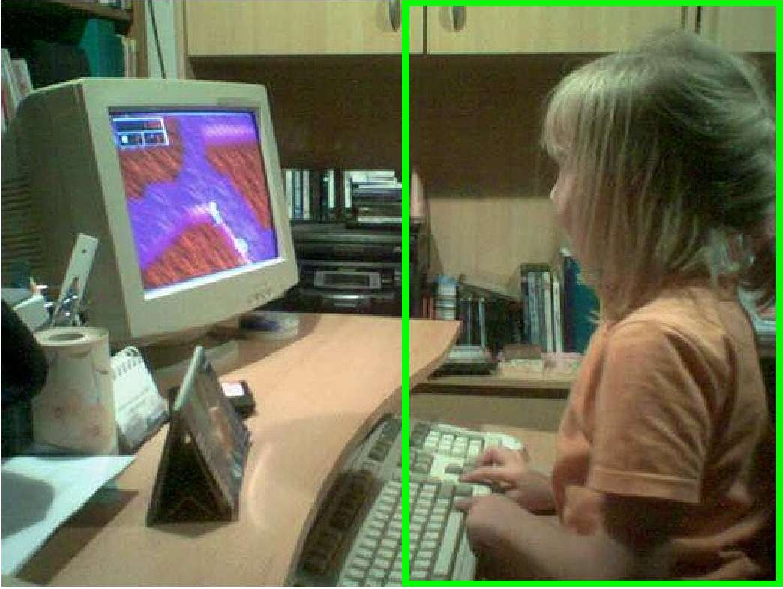
\includegraphics[height=0.12\textwidth,width=0.15\textwidth]{person_pos_000421.pdf}&
  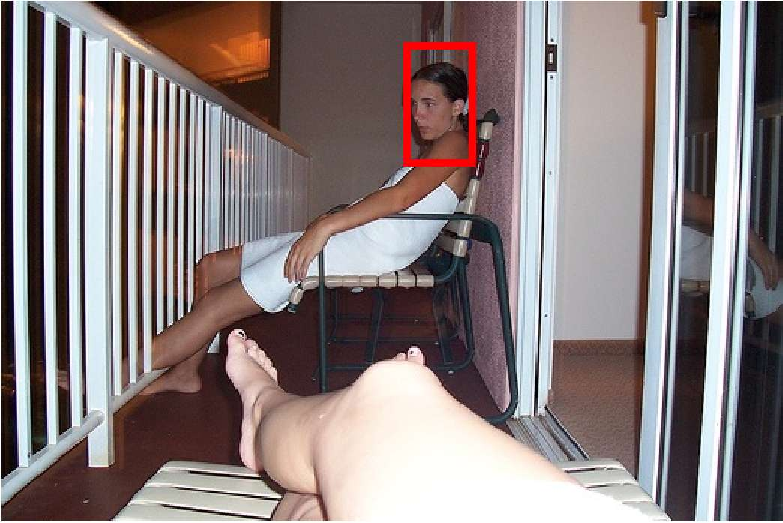
\includegraphics[height=0.12\textwidth,width=0.15\textwidth]{person_neg_000090.pdf}\\[-2ex]
  
  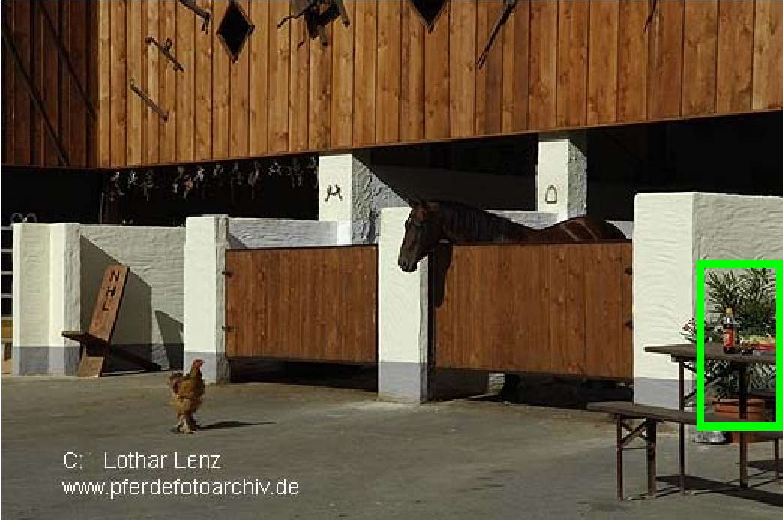
\includegraphics[height=0.12\textwidth,width=0.15\textwidth]{plant_pos_000737.pdf}&
  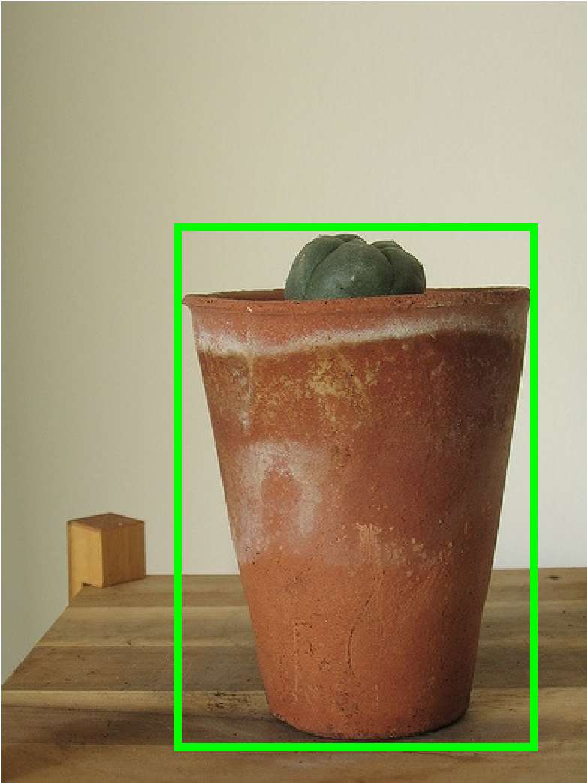
\includegraphics[height=0.12\textwidth,width=0.15\textwidth]{plant_pos_000933.pdf}&
  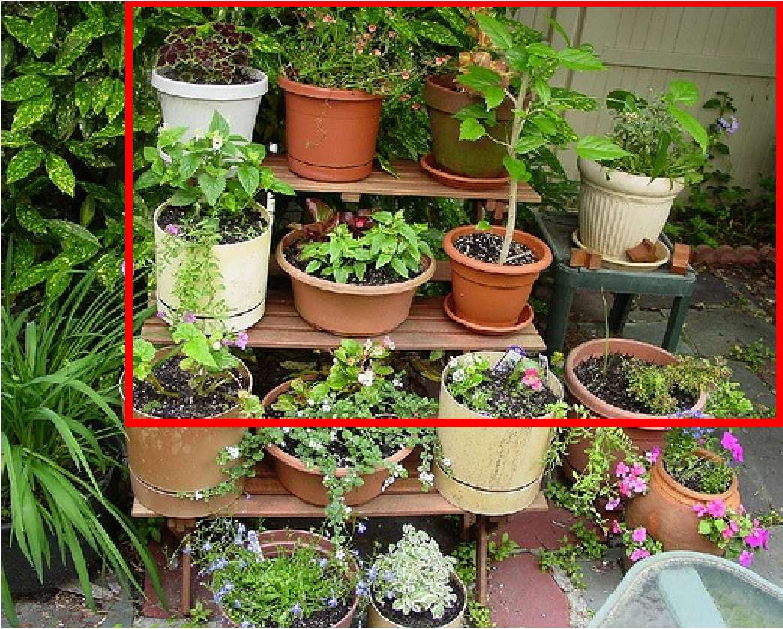
\includegraphics[height=0.12\textwidth,width=0.15\textwidth]{plant_neg_001070.pdf}&
  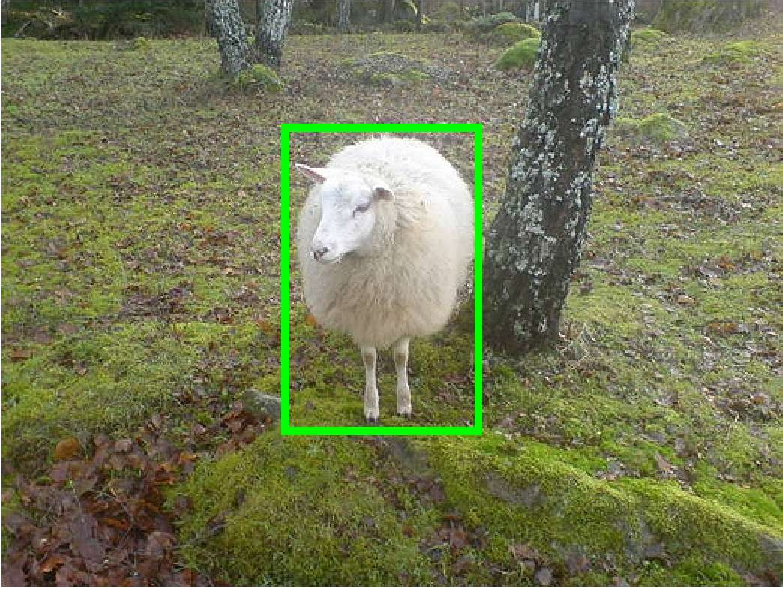
\includegraphics[height=0.12\textwidth,width=0.15\textwidth]{sheep_pos_000779.pdf}&
  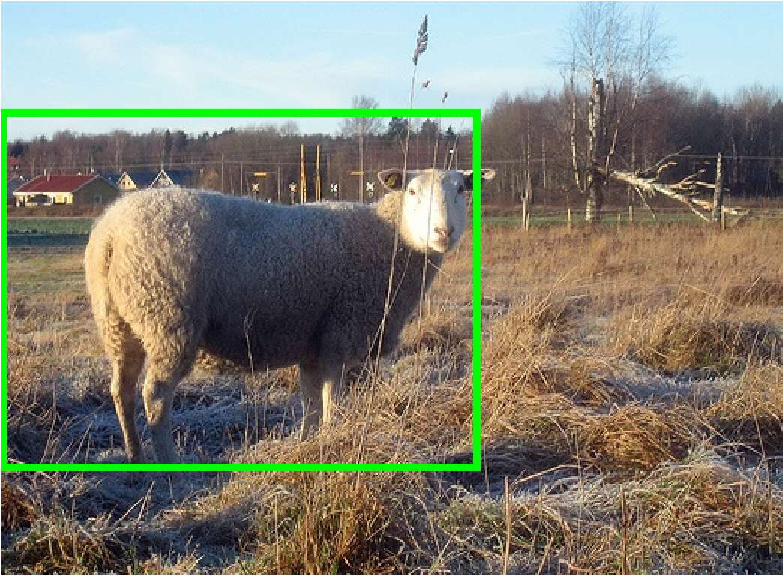
\includegraphics[height=0.12\textwidth,width=0.15\textwidth]{sheep_pos_000627.pdf}&
  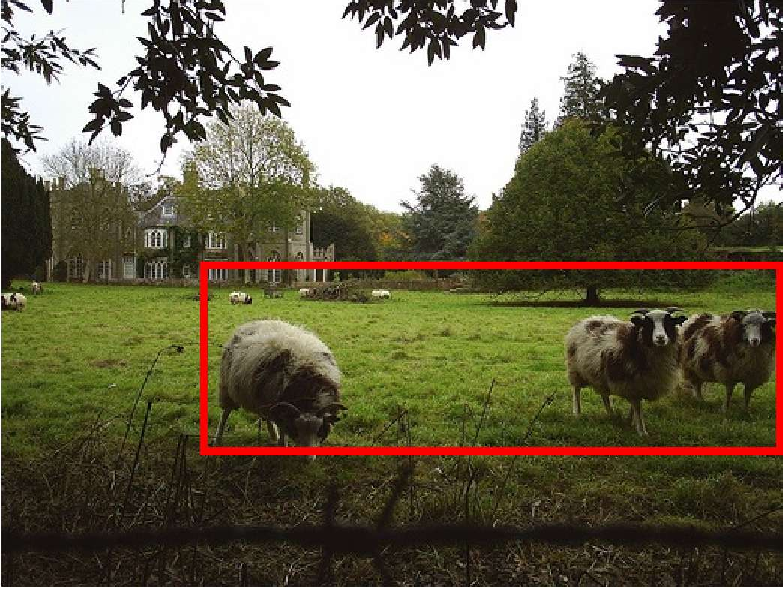
\includegraphics[height=0.12\textwidth,width=0.15\textwidth]{sheep_neg_000992.pdf}
  \end{tabular}
% \end{center}
\caption{This figure depicts success (in green) and failure cases (in red) of our detector in randomly picked images. Majority of false detections contains two kinds of error: i) group multiple object instances with a single bounding box, ii) focus on (discriminative) parts (\eg ``faces'') rather than whole object. }
\label{fig:detexamples}
\end{figure*}


% --------------------------------------------------------------------------------------
\subsection{Classification Results}
% --------------------------------------------------------------------------------------
While WSDDN is primarily designed for weakly-supervised object detection, ultimately it is trained to perform image classification. Hence, it is interesting to evaluate its performance on this task as well. To this end, we use the PASCAL VOC 2007 benchmark and contrast it to standard fine-tuning techniques that are often used in combination with CNNs and show the results in \cref{tab:voc2010corloc}. These techniques have been thoroughly investigated in~\cite{Chatfield14,He14,Oquab14}. Chatfield \etal~\cite{Chatfield14}, in particular, analyse many variants of fine-tuning, including extensive data augmentation, on the PASCAL VOC. They experiment with three architectures, VGG-F, VGG-M, and VGG-S. While VGG-F is their fastest model, the other two networks are slower but more accurate. As explained in \ref{subsec:expsetup}, we initialise WSDDN \textbf{S} and \textbf{M} with the pre-trained VGG-F and VGG-M-1024 respectively and thus they should be considered as right baselines. WSDDN~\textbf{S} and \textbf{M} improves $~8$ and $~7$ points over VGG-F and VGG-M-1024 respectively. 


We also compare WSDDN to the SPP-net \cite{He14} which uses the Overfeat-7 \cite{Sermanet13} with a 4-level spatial pyramid pooling layer $\{6\times 6, 3\times 3, 2\times 2, 1\times 1\}$ for supervised object detection. While they do not perform fine-tuning, they include a spatial pooling layer. Applied to image classification, their best performance on the PASCAL VOC 2007 is $82.4\%$. Finally we compare WSDDN~\textbf{L} to the competitive VGG-VD16~\cite{Simonyan15}. Interestingly, this method also exploits coarse local information by aggregating the activations of the last fully connected layer over multiple locations and scales. WSDDN~\textbf{L} outperforms this very competitive baseline with a margin of $0.4$ point.

